\documentclass[11pt]{article}
% guidelines at http://tab.computer.org/tcde/bull_author.html
\usepackage{deauthor,times,graphicx}
%\graphicspath{{authorname/}}

%\usepackage[dvipsnames,svgnames]{xcolor}
\usepackage{tikz}
\usepackage{amssymb, framed}
\usepackage{tikz}
\usepackage{rotating}
\usepackage{xcolor}
\usepackage{hyperref}
\usetikzlibrary{trees,shapes,snakes,patterns}
% % % --------------------------------------- % % %
% % % Macros to write comments for internal usage % % %
% % % --------------------------------------- % % %

\newcommand{\red}[1]{\textcolor{red}{#1}}
\newcommand{\eat}[1]{}
\newcommand{\argmax}{\mathop{\rm arg~max}\limits}

\begin{document}
\title{%How AI and People Work Together: 
Computational Division of Labor with Human and AI Workers}
%The future of Crowdsourcing Platforms: Ecosystems and Interoperability}

%\author{Atsuyuki Morishima,\\ University of Tsukuba\\
%\texttt{{\footnotesize mori@slis.tsukuba.ac.jp}}
%\and
%Masaki Matsubara\\
%University of Tsukuba\\
%\texttt{{\footnotesize masaki@slis.tsukuba.ac.jp}}
%\and
%Kei Wakabayashi\\
%University of Tsukuba\\
%\texttt{{\footnotesize kwakaba@slis.tsukuba.ac.jp}}
%\and
%Nobutaka Suzuki\\
%University of Tsukuba\\
%\texttt{{\footnotesize nsuzuki@slis.tsukuba.ac.jp}}
%\and
%Hiroyoshi Ito\\
%Universityu of Tsukuba\\
%\texttt{{\footnotesize ito@slis.tsukuba.ac.jp}}
%}

\author{
	Atsuyuki Morishima,
	Masaki Matsubara,
	Kei Wakabayashi,
	Nobutaka Suzuki,
	Hiroyoshi Ito \\
	University of Tsukuba\\
	\texttt{{\footnotesize \{mori, masaki, kwakaba, nsuzuki, ito\}@slis.tsukuba.ac.jp}}
}

\maketitle

\newcommand{\scream}[1]{\textbf{***#1***}}

% -------------------------------------------------------- %

\begin{abstract}
Online crowdsourcing platforms have proliferated over the last few years and cover a number of important domains, these platforms include from worker-task platforms such Amazon Mechanical Turk, worker-for-hire platforms such as TaskRabbit to specialized platforms with specific tasks such as ridesharing like Uber, Lyft, Ola etc.
An increasing proportion of human workforce will be employed by these platforms in the near future.
The crowdsourcing community has done yeoman's work in designing
effective algorithms for various key components, such as incentive design, task assignment and quality control. Given the increasing importance of these crowdsourcing platforms,
it is now time to design mechanisms so that it is easier to evaluate the effectiveness of these platforms. Specifically, we advocate developing benchmarks for crowdsourcing research.

Benchmarks often identify important issues for the community to focus and improve upon.
This has played a key role in the development of research domains as diverse as
databases and deep learning.
We believe that developing appropriate benchmarks for crowdsourcing will ignite further innovations.
However, crowdsourcing -- and future of work, in general -- is a very diverse field
that makes developing benchmarks much more challenging.
Substantial effort is needed that spans across developing benchmarks for
datasets, metrics, algorithms, platforms and so on.
In this article, we initiate some discussion into this important problem and
issue a call-to-arms for the community to work on this important initiative.
\end{abstract}

\section{Introduction}
\label{sec:intro}

Federated Learning (FL) is a distributed machine learning (ML) paradigm that trains a model across a number of participating entities holding local data samples.
% , without exchanging them. 
In this work, we focus on \emph{cross-device} FL that harnesses a large number (up to hundreds of millions) of edge devices with disparate characteristics such as availability, compute, memory, or connectivity
resources~\citep{kairouz2019advances}. %that harnesses potential
% Current applications of FL are designed to scale up to client populations of hundreds of millions or even billions. 
Two challenges to the success of cross-device FL are privacy and scalability. 
FL was originally motivated for improving privacy since data points remain on client devices. 
% and only small model updates were shared to a co-ordinating server.
However, as with other forms of ML, information about training data can be extracted via membership inference or reconstruction attacks on a trained model \citep{carlini2021membership,carlini2020extracting}, or leaked through local updates~\citep{MelisSCS19,geiping2020inverting}. 
Consequently, Secure Aggregation (\SecAgg) protocols were introduced to prevent the server from directly observing individual client updates, which is a major vector for information leakage~\citep{bonavitz2019federated,huba2021papaya}. 
Additional mitigations such as  Differential Privacy (DP) may be required to offer further protection 
against attacks~\citep{dwork2006calibrating,abadi2016deep}, as discussed in Section~\ref{sec:discussion}.
% , as discussed in Section~\ref{sec:discussion}.
%As an additional layer of protection against statistical inference attacks, SecAgg is usually paired with Differential Privacy (DP) \citep{dwork2006calibrating}. To realize the full promise of FL as a privacy-enhancing technology, we need both SecAgg and Differential Privacy.

Ensuring scalability to populations of heterogeneous clients is the second challenge for FL.
% There are many aspects for FL scalability, such as ensuring that model updates can be calculated efficiently 
% by devices with various capabilities and intermittent availability~\citep{bonavitz2019federated}.
% Here, we focus on the communication bottleneck as the primary concern.
Indeed, wall-clock training times are highly correlated with increasing model and batch sizes~\citep{huba2021papaya}, even with recent efforts such as FedBuff~\citep{nguyen2021federated},
% With increasing model and batch sizes, the wall-clock training time increases accordingly~\citep{huba2021papaya}. 
% Despite efforts such as buffered asynchronous aggregation~\cite{nguyen2021federated}, 
and communication overhead between the server and clients dominates model convergence time.
% cross-device FL remains bottlenecked by communication latency between the server and the clients. 
% \karthik{should we mention this paper in a different way? Fedbuff paper doesn't explicitly call out latency as an issue, nor do we run experiments to on async fl ourselves}  \ashkan{I also think the transition can be smoother: first we focus on scalability and billions. Then we say communication is the bottleneck} 
Consequently, compression techniques were used to reduce the communication bandwidth while maintaining model accuracy.
However, a fundamental problem has been largely overlooked in the literature: in their native form, standard compression methods such as scalar quantization and pruning are not compatible with \SecAgg. 
This makes it challenging to ensure both security and communication efficiency.
% at the same time.
% the default method to provide security for client update, 
% presenting an unpleasant dichotomy between security or efficiency. 


% Second, this is the most restricted direction, since upload bandwidth remains more restricted than download. 
% In the US, fixed-line broadband speeds typically achieve a ratio of $3\times$ to $20\times$ more download bandwidth than upload
% bottlenecks remain, and so we seek to reduce the message size of clients by \textit{compression}. 
% Compression has been widely proposed in various ML scenarios, in the form of pruning (removing model parameters) and quantization (reducing fidelity of parameter representation). 
% Indeed, these techniques have been successfully used in FL settings with appreciable improvements in communication while maintaining model accuracy. 
% However, there is a fundamental problem which has been largely overlooked in the literature: in their native form, these compression methods are not compatible with SecAgg, the default method to provide security for client updates. 
% This presents an unpleasant dichotomy: we can have security or efficiency, but not both. 
%
%
% In this paper, we resolve this gap by showing how to modify FL compression techniques to make them security-friendly. We focus on compressing \emph{uplink} updates from clients to the server for two reasons. 
% First, uplink communications are subject to Secure Aggregation protocols to ensure a high security bar, while downlink updates broadcasted by the server are deemed public. 
% Second, upload bandwidth is generally more restricted than download. For instance, according to the most recent FCC report, the ratio of download to upload speeds for DSL/cable providers\footnote{Fixed-line broadband is most relevant since FL is typically restricted to using unmetered connections, usually over Wi-Fi~\citep{huba2021papaya}.} in the US ranges between 3$\times$ to 20$\times$~\citep{fcc-broadband}.
% % This requires some meticulous changes to coordinate clients to use the same global (non-private) hyperparameters, and show that this coordination does not damage model quality. 
% % For the strongest compression methods, we step outside of the SecAgg primitive and propose a new secure primitive, Secure Indexing, which enables the best compression ratios without sacrificing utility. 
% Finally, efficient and secure uplink communication brings several benefits beyond speeding up convergence: 
% lowering communication cost reduces selection bias due to undersampling clients with limited connectivity, improving fairness and inclusivity metrics. 
% It also shrinks the carbon footprint of FL, whose fraction attributable to communication can reach 95\%~\citep{qiu2021first}.
%
%In this paper, w
We address this gap by adapting compression techniques to make them compatible with \SecAgg. We focus on compressing \emph{uplink} updates from clients to the server for three reasons. 
First, uplink communication is more sensitive and so is subject to a high security bar, whereas downlink updates broadcast by the server are deemed public. 
Second, upload bandwidth is generally more restricted than download bandwidth. For instance, according to 
a recent FCC report, 
%the most recent \modif{FCC\footnote{\modif{US Federal Communications Commission.}} report}, 
the ratio of download to upload speeds for DSL and cable providers\footnote{FL is typically restricted to using unmetered connections, usually over Wi-Fi~\citep{huba2021papaya}.} in the US ranges between 3$\times$ to~20$\times$~\citep{fcc-broadband}.
% Fixed-line broadband is most relevant since
% This requires some meticulous changes to coordinate clients to use the same global (non-private) hyperparameters, and show that this coordination does not damage model quality. 
% For the strongest compression methods, we step outside of the SecAgg primitive and propose a new secure primitive, Secure Indexing, which enables the best compression ratios without sacrificing utility. 
Efficient uplink communication brings several benefits beyond speeding up convergence: 
lowering communication cost reduces selection bias due to under-sampling clients with limited connectivity, improving fairness and inclusiveness. 
It shrinks the carbon footprint of FL, the fraction of which attributable to communication can reach 95\%~\citep{qiu2021first}.
In summary, we present the following contributions: 
\begin{itemize}
    \item We highlight the fundamental mismatch between two critical components of the FL stack: \SecAgg protocols and uplink compression mechanisms.
    
    \item We formulate solutions by imposing a linearity constraint on the decompression operator, as illustrated in Figure~\ref{fig:secagg_summary} in the case of TEE-based \SecAgg.
    
    \item We adapt the popular scalar quantization and (random) pruning compression methods for compatibility with the FL stack that require no changes to the \SecAgg protocol.
    
    \item For extreme uplink compression without compromising security, we propose Secure Indexing (\SecInd), a variant of \SecAgg that supports product quantization. %and admits a secure implementation.
\end{itemize}

\begin{figure*}[t]
    \centering
    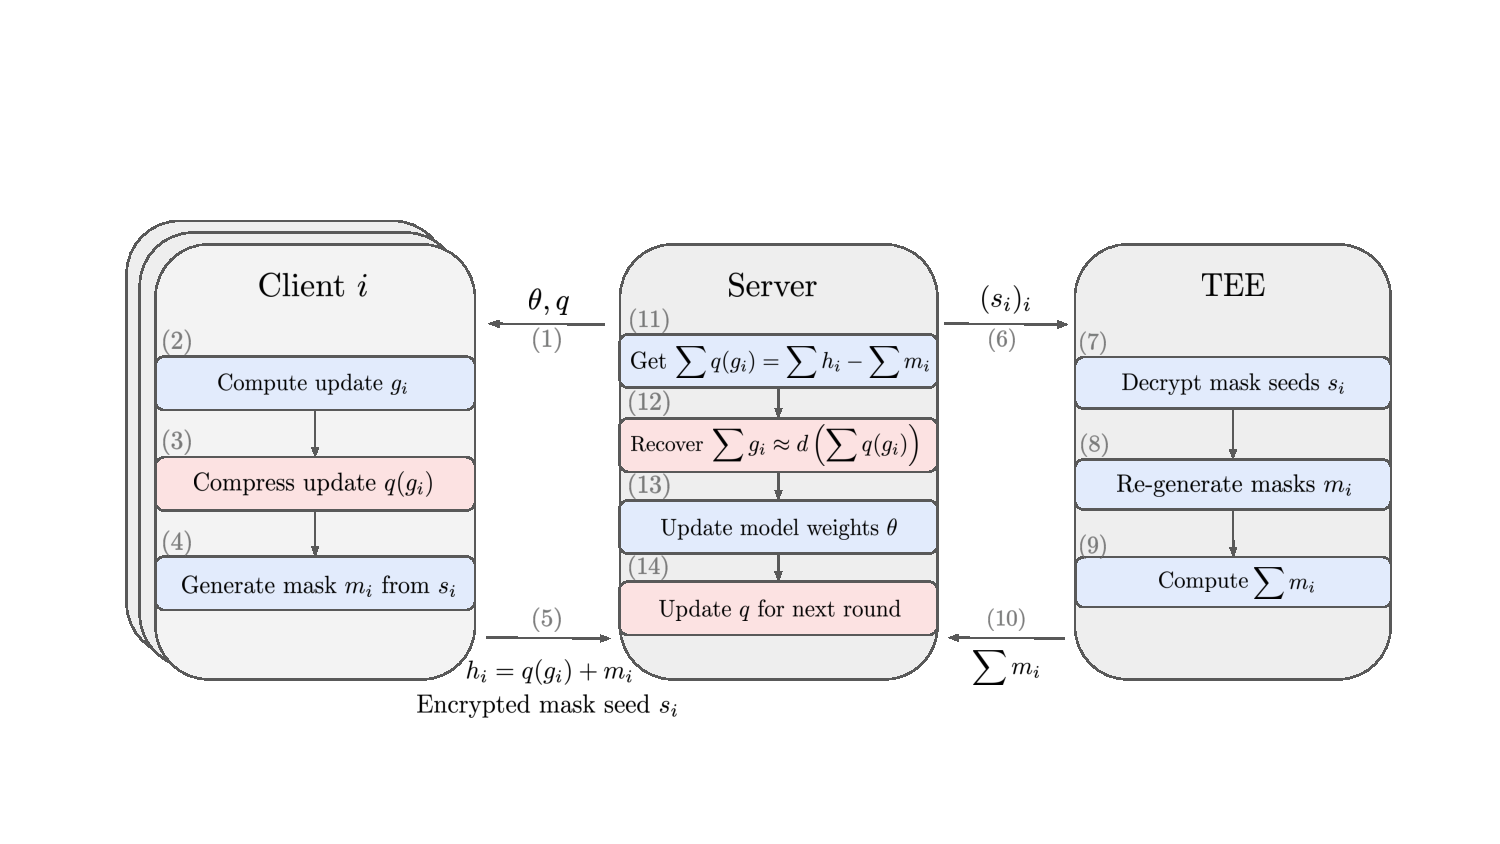
\includegraphics[width=0.8\textwidth]{figs/secagg_summary_new.pdf}
    %\vspace{-5mm}
    \caption{\label{fig:secagg_summary}
    Summary of the proposed approach for one FL round, where we omit the round dependency and \modif{Differential Privacy (DP)} for clarity. Blue boxes denote standard steps and red boxes denote additional steps for uplink compression. Client $i$ computes local model update $g_i$, compresses it with the compression operator $q$, and encrypts it by adding a random mask $m_i$ in the compressed domain, hence reducing the uplink bandwidth (steps 2--4). The server recovers the aggregate in the compressed domain by leveraging any \SecAgg protocol \modif{(steps 7--13, with a TEE-based \SecAgg, see Section~\ref{subsec:secagg})}. Since the decompression operator $d$ is linear, the server can convert the aggregate back to the non-compressed domain, up to compression error (step 12). As with the model weights $\theta$, the compression operator $q$ are also periodically updated and broadcast by the server (step 14). 
    In Section~\ref{sec:method}, we apply the proposed method to scalar quantization and pruning without impacting \SecAgg and propose Secure Indexing, a variant of \SecAgg for extreme uplink compression with product quantization. See Section~\ref{subsec:secagg} for details about \SecAgg and Section~\ref{sec:discussion} for a discussion on~DP.
    }
    \vspace{-3mm}
\end{figure*}



% Our focus in this paper is on 

%Second, scaling cross-device (synchronous) FL to millions of clients with various capabilities and intermittent availability \citep{bonavitz2019federated} suffers from diminishing returns: the wall-clock training time plateaus as the number of clients keeps increasing~\citep{huba2021papaya}. Even though this challenge can be addressed by leveraging the buffered asynchronous aggregation technique proposed by \cite{nguyen2021federated}, compatible with DP and SecAgg, the asynchronous protocol remains bottlenecked by communication latency between the server and the clients.


%Considering the above privacy and scalability goals, we focus on enabling efficient FL communications while keeping a high privacy bar. In addition to the primary objective of speeding up convergence, reducing communication costs brings other significant benefits. Lowering communication requirements addresses selection bias due to undersampling clients with limited connectivity, improving fairness and inclusivity metrics. Better communication efficiency shrinks the carbon footprint of FL, whose fraction attributable to communication can reach 95\%~\citep{qiu2021first}. %Finally, training larger model in FL would be a possibility, when the communication cost is reduced, because local memory or compute requirements can be addressed by modifying the local training loop, for instance with gradient checkpointing \citep{chen2016training}. However, some form of compression would be required to enable efficient communication.


%First, compressing model updates from the client to the server presents several challenges due to compatibility with SecAgg and is an area suitable for further research. 
%Second, upload bandwidth is generally more restricted than download. For instance, according to the most recent FCC report, the ratio of download to upload speeds for DSL/cable providers in the US ranges between 3$\times$ to 20$\times$~\citep{fcc-broadband}. We consider broadband speeds here because devices participate in the FL training while connected to fixed broadband, usually through Wi-Fi~\citep{huba2021papaya}.




% Hence, FL provides the ability to leverage data from massive client populations while ensuring the security and privacy of the client data.
% Go further: compatibility with DP / compression as a mitigation techniques of attacks
% Model and gradient compression intrinsically different.
%  Why not having the secure enclave perform the aggregation?
%
%!TEX root = ../main.tex
 
\section{AI-Native Database}
\label{sec:ANDB}
 
%\subsection{Motivation}\label{sec:motivation}
 

We aim to study how AI and DB can benefit from each other. Firstly, we discuss how AI technique can benefit databases (AI4DB). Secondly, we present how database techniques can help AI (DB4AI). Thirdly, we discuss how to fully utilize the new hardware to support both AI and DB. 


\subsubsection{AI4DB}
AI techniques can benefit databases from six aspects.

\hi{Self-configuration.} All databases have hundreds of tuning knobs, which are vital to nearly every aspect of databases, such as performance, availability, robustness, etc. However, these configurations require to be adjusted manually, which not only is time consuming but also cannot find optimal configurations. AI based methods, e.g., deep reinforcement learning, can automatically tune the database knobs. Moreover, other configurations (e.g., software bugs, partition scheme) can also be optimized by AI-based methods. 


\hi{Self-optimizing.} AI can optimize the database performance from many aspects. First, cost/cardinality estimatio is vital to query plan selection. However, database mainly estimates cardinality based on raw statistics (e.g., read/write blocks, backends, deadlocks) and is poor in estimating the resulting row number of each query operator (e.g., hash join, aggregate, filter), with histograms simply. AI-based methods, e.g., Tree-LSTM, can learn data distribution in depth and provide more accurate cardinality estimation. Second, join order selection. Different join schemes have a great impact on query efficiency. And finding the best plan is a NP-hard problem. With static algorithms (e.g., dynamic programming, heuristics algorithm), the performance of join order selection in database is limited by the effect of the estimator. AI based methods can better choose between different join order plans by taking one-step join as the short-term reward and the execution time as the long-term reward. 

\hi{Self-healing.} High reliability within database has become a critical requirement. But database can crash down for many reasons (e.g., poor performance, hardware/software failovers). So to keep database running is a tough thing. Attempts of traditional database include two aspects. First, set rule-based monitors and alert people when trigger the threshold. But the standards are coarse-grained and cannot effectively prevent accidents. Second, back up data or image periodically. Although that can help in recovery, it cannot assure high reliability. AI-based methods, e,g, CNN, can automatically detect, diagnose, alert and recover from database problems. For example, for distributed database, it supports live data migration when nodes crash or load leans with minimum cost. 

\hi{Self-protecting.} High availability is another important requirement. Database needs to protect the health of each transaction, such as the waiting time and the allocated resources.  Without dynamic protecting mechanisms, database performance can be affected. First, unhealthy resource competition can severely affect database stability. AI-based methods can automatically balance the relation between workspace of a single query and the overall concurrency. Second, anomaly query can cause great loss to database. For example, run-away queries take much longer time than estimated in query plan, which may be hanging. And database will execute such queries for very long time before kill them. With AI techniques, we can not only solve the problems in query processing, but avoid wasting resources for run-away queries.

\hi{Self-inspecting.} Data consistency is vital to data validation. Database maintains data consistency with fixed rules. For example, for single database, data in memory is written back to disk every a number of write operations; for distributed database, data is synchronized between replication nodes using writing logs. With AI techniques, database can automatically learn how to check and assure data consistency and database health. To a higher level, AI models should translate those experiences into publication of instrumentation to help human beings understand.

\hi{Self-assembling}. Each processing layer (e.g., optimizer, executor, storage engine) in a database has several alternatives, each of which has its own advantages. But in traditional database, query is processed in fixed path and cannot take advantage of optional components dynamically. With AI techniques, it can learn how to select proper component in each layer and assemble the complete executing path based on the query and workload characters.


%With AI techniques, the AI model can help in three ways. 1) It can tune automatically. With advanced learning algorithms such as backward propagation, it can tune even better than DBA; 2) It can tune dynamically. Taking environment and workload as input, it can be aware of changes in workload and environment (e.g., hardware migration, various workloads) and tune dynamically.

%\lgl{Self-optimizing.} AI can optimize the database performance from many aspects. First, cost/cardinality estimation ad join order selection are b  database optimizer relies on . 

%Thirdly, database cannot optimize itself dynamically. Optimizer in traditional database cannot assure the performance of the query plan. 1) Database is poor in cardinality estimation, which is vital to query plan selection. Traditionally database mainly collects raw statistics (e.g., read/write blocks, backends, deadlocks) and is poor in estimating the resulting row number of each query operator (e.g., hash join, aggregate, filter) with histograms. With AI techniques, neural network can learn data distribution in depth and provide more accurate cardinality estimation. 2) Database cannot automatically design auxiliary structures (e.g., indexes, materialized views/query tables) to optimize the performance of queries. With AI techniques, the AI model can automatically analyze history workload information and pre-build those structures. For example, DDQN model can learn and predict the features of incoming queries and pre-build indexes on proper columns to accelerate the execution of queries.




%Firstly, data is explosively growing. Since 2010, data has been dramatically increasing, at a rate of doubling every two years. And it is expected to hit 45,000 exabytes in 2020. 
%Explosive data growth has exposed many problems in existing databases. 
%1) Traditional manual tuning methods can no longer meet our needs. Proper configuration is important to database performance. And in cloud, it is impossible for DBAs to manually tune each database instance. So we need to combine AI tech to automate this work.
%2) For distributed database, it has many mechanisms (e.g., data sharding and load balancing) to ensure the performance does not degrade. But those components usually adopt simple strategies, whose error rate is high and can seriously affect the performance. For example, in data sharding, chunks of the same table can have different access frequency. And by evenly distributing data among the nodes some nodes can be overloaded or even crash, while others are idle. So we hope to use AI model to monitor, analyze and maintain load balancing at all times.
%3) The traditional database components such as query optimizer and index building struggle with big data. For example, using simple heuristic algorithm, the optimizer can recommend terrible query plan and waste unaffordable time and resources to execute it. So we hope to use AI algorithm to generate proper query plan within acceptable time.

%Secondly, enterprises have entered the era of integrated data analysis (IDA), in which two or more independent data sets are pooled or combined into one and then statistically analyzed. IDA is costly to conduct.
%1) Different data is stored in different databases. For example, we store highly structured data in relational databases, streaming data in time-series databases and graph data in graph databases. And current database has fixed schemas. So it's expensive to aggregate data from different databases.
%2) Schema is different. Structured data is stored in well-defined schema and is easy to manipulate with SQL.
%Although unstructured data also has internal structure, it is of complex data forms (e.g., e-mails, digital images and navigation details) and is not suitable to be reshaped with pre-defined data models. To force these two kinds of data into the same schemas can lead to great information loss or resource waste.
%emails, text files, web pages, digital images, multimedia content, navigation details and social media posts.


\subsubsection{DB4AI}
AI techniques rely on data heavily. With database storing, managing and manipulating data, the training and learning procedure can be more efficient. But to support AI techniques on database, there are several problems. 
% For any AI technique, it needs large volume of data for model training.

Firstly, AI has different user interfaces to DB. Generally, people write AI models in Python or R languages, but manipulate data from relational database with SQL statements. There are two problems when call AI-related services. 1) People need frequently switch between different systems when writing AI-related applications. 2) It is not easy for traditional data analysts, who only know some SQL knowledge, to write AI code. So if we can extend parsing rules to make SQL support both DB and AI, it would be very convenient to support AI-related  services.

Secondly, DB can optimize AI algorithms. Database can not only provide AI with data, but better support AI services with its mechanisms. We can see from model building training, reusing. 1) With unified SQL interface, user can easily build an AI model using user defined functions or stored procedures. 2) Training AI models consume time with a large number of tensor calculation. Database can better support tensor operators with extended relational algebra and execute them in the executor, which help in model training. 3) Well-trained AI models can be persisted with materialized views or query tables and be reused easily and efficiently.


%they have different data models. For DB, techniques (e.g., CRUD, data integration and data management) are based on relational data model, with which we conduct operations such as join and aggregate. For AI, models (e.g., traditional machine learning, deep learning, reinforcement learning) are based on tensor data model, with tensor operators such as tensor product, addition and division. So the overhead to convert DB data into AI data is relatively high. And we know that, for an AI model, data preprocessing takes most code and wastes much training time. Currently, no practical system can unify these two data models within a single system.

\subsubsection{Heterogeneous Computing Framework}

With Moore's law on the verge of failure, database can no longer rely on single processor to improve processing ability. Now heterogeneous computing framework brings about new potential. Firstly, it incorporates different computing powers (e.g., GPU, NPU, FPGA) and accelerators. Secondly, with dissimilar co-processors handling different tasks, it can gain great improvement in performance and efficiency. But to support heterogeneous computing framework, database needs to solve three main problems.

	$\bullet$ Single resource scheduling in system level. The theoretical architecture and operators in traditional DB are not suitable to computing-intensive chips. That is, simple computing in structured data analysis dose not need chips with high parallel computing power. DB needs to design special heterogeneous computing units, considering of computing and storing resources.

	$\bullet$ Single accelerator architecture. Traditional accelerator architecture only supports OLAP type, For OLTP and HTAP workloads, caused by data consistency between system memory and accelerator's local memory, it is inefficient. DB needs to incorporate new techs, such as CXL released by Intel, to provide efficient memory access methods for accelerators.

	$\bullet$ Single relational algebra. Firstly, to provide heterogeneous computing, we need to define data models for different operating. For example, relational data model is good for data management, but cannot fit TPU/NPU processing model. Besides, We want different computing powers to work together. For example, with extended relational algebra, we can use tensor computing model to accelerate relational operators, such as join and aggregation.


%For example, with the parallel computing design, GPU is good at large-scale data computation, which can efficiently save the training time of neural networks.


%\section{Platform Design}
\label{sec:platformDesign}

Based on the analysis of the poll of crowd workers
and extensive discussions with participants of the 2019 Shonan Seminar on Future of Work\footnote{ACM Sigmod Blog, Sept. 23, 2019,  \url{http://wp.sigmod.org/?p=2931}},
we have identified platform design as one of the key drivers
for ensuring the continued success of online job platforms.
We first identify a number of issues with the current platform design and make a number of concrete suggestions.

\textbf{Lack of Interoperability:}
The current generation of online job platforms operates in silos.
Even platforms that are in a specific domain such as driving (Uber, Lyft, Ola, Didi, etc.) are not
interoperable with each other.
A driver who has driven more than 10K rides with 4.9 rating in Uber will start
as a newbie when moving to a different platform such as Lyft.
This is also a problem for requesters. Consider a task that requires 10 experts.
It is possible that the labor market has the requisite experts -- but they are scattered across multiple platforms.
In this case, the requester could not successfully complete the task.
By enabling interoperability between platforms such issues and many more could be ameliorated.

\textbf{Lack of Support for Complex Tasks and Workflows:}
Currently, there are a limited number of tasks for which crowdsourcing is possible.
Even sophisticated platforms such as CrowdWorks only support as little as 200 types of tasks.
As more and more task types are being serviced by gig economy,
the need for supporting more complex tasks becomes important.
These complex tasks often have very different set of requirements.
For example, they might require a sophisticated workflow so that output of one stage is passed to another. They could require workers with different types of roles.
There might also be a need for specialized requirements such as splitting
a complex task into multiple sub-tasks that could then be assigned using a workflow.


\textbf{Limited Pricing Model:}
There are four types of pricing  models that are widely prevalent in online job platforms.
First is the fixed income model where each worker is given a fixed amount of money every month or so.
There is also task based pricing where the worker is paid a pre-agreed amount after completing a task.
There are some intermediate approaches such as fixed income plus a bonus amount and discounted pricing for completing large number of tasks.
Finally, there are competitions pricing  models in which we pay to the winner.
For online job platforms to thrive, it is important to have a wider variety of pricing models.

For the remainder of the section, we propose a number of improvements to platforms
that could either reduce the pain points of the key stakeholders or improve their satisfaction.

\subsection{Platform Design for Workers}
Workers are the back bone of a job platform by completing the tasks of requesters.
As discussed in the previous section, the current generation of platforms are not very conducive for
long term employment.

\textbf{Ease of On- and Off-boarding:}
One of the positive things about online job platforms is the flexibility they provide to the worker.
The worker can take tasks that are of interest to them while operating flexible hours.
Many platforms simplify them with as little as some identity document and bank account.
While joining the platform is straightforward, the onboarding process often leaves much to be desired.
Once the worker joins the platform, they are not provided enough guidance to contribute productively.
The worker is expected to learn how to contribute on their own.
Similar to offline employment in a traditional organization, it is important to have a proper onboarding procedure.
The current process for off-boarding is also ad-hoc.
Typically, workers and requesters can easily stop working in a platform.
However, the workers often lose the reputation that they have earned when moving to a different platform.
Similarly, the requesters also lose access to valuable and productive employees when moving to a different platform.
It is important to have a better off-boarding platforms so that the workers could transfer the reputation and knowledge learned from one platform to another.

\textbf{Support for Learning Skills.}
When a worker joins a platform, she often learns ``on-the-job''.
If the worker does not perform well due to inexperience, the job could be rejected by the requester
thereby affecting the approval rate of the worker.
Since a number of requesters filter workers based on task approval rate,
this could limit the number of tasks a new worker could contribute to.
This often leads to frustration of new workers and eventual turnover.
It is often desirable to have a more formal mechanism for simplifying this process.
For example, job platforms could have a collection of previously completed tasks
that could serve as an on-ramp for the workers.
By working on such tasks, the worker can learn the requisite skill in a low stress environment.


\textbf{Knowledge Base (KB) for Workers:}
Currently, there are a number of knowledge repositories in an
enterprise so that employees know the practices of the company.
It is important that online job platforms provide something similar.
Note that this is in addition to the aforementioned set of completed tasks.
As workers finish tasks, they must be able to add things to a personalized knowledge base
about what they learned from the task.
This could be public so that any worker can learn from it or
private where it is visible only to the worker.
As workers become increasingly knowledgeable, this serves as a repository for what they learned over the years.
Of course, this must also be interoperable and associated with the worker and transferable as needed.
This will also allow workers to find other mentors or experts to learn from.

%\scream{I moved Support of AI worker to the next session and added the following paragraph.}

\textbf{Support for Expressing Workers' Preference on Task Assignment}
The task assignment is usually done by workers themselves, partly because automatic assignment of  tasks to workers is not straightforward. There are many reasons for the worker to do the tasks; they did the task because it was easy to do, the task was interesting, they wanted to learn something from the task,  it gave them a lot of money, or it was the regular time slot for the worker to do tasks. If the platform has  the support for them to express their preferences, platforms will be able to automatically suggest them the tasks more accurately.






\subsection{Platform Design for Requesters}
In this subsection, we highlight some of the major pain points of requesters
and how new functionality from platforms could improve their satisfaction.

\textbf{Expressive Specification of Task Requirements.}
Currently, there is limited support from online job platforms for requesters
to precisely specify their requirements.
For example, in AMT, the requester can filter workers based on approval rate but cannot impose additional sophisticated filtering.
It is important for requesters to be able to specify worker requirements such as skills~\cite{DBLP:conf/www/MavridisGM16},
output requirements such as latency, cost and quality.
Furthermore, the requester could be open to various tradeoffs such as cost vs quality / latency.
For example, one might be willing to pay higher for better quality or faster response.
Unfortunately, current platforms do not provide such flexibility.

\textbf{Supporting Complex Tasks and Workflows.}
Almost all of the current job platforms support simple microtasks.
As more and more tasks are disrupted by the gig economy, it is important to have platforms that can support more complex tasks.
Often, complex tasks have a number of distinct requirements.
They are often knowledge intensive and collaborative~\cite{rahman2015task} requiring co-ordination with multiple workers.
They often are not monolithic and must be split into multiple sub-tasks
with different groups of workers completing each of them.
They also often require workers to embrace different roles.
Finally, they often have a complex workflow where the output of one stage is passed to the next.

\textbf{Support for Workflow Evolution and Changes during the Execution.} Workflows sometimes
need to change or evolve during the execution, since completing all tasks requires a long time in
general and it is often the case that we find better workflows after we start to execute the
original workflow. The platforms should support this kind of evolution and changes of workflows
with a minimum amount of effort.

\textbf{Sophisticated Algorithms for Assigning Workers to Tasks.}
Currently, most crowdsourcing platforms do not have
any sophisticated algorithms in matching workers to tasks.
Often, this is done manually by the workers by browsing the list of available tasks.
Other than filtering the pool of workers, requesters do not have much control on which workers perform the tasks.
Despite extensive research in algorithms for task assignment~\cite{basu2015task,ho2012online,rahman2015task},
they are not often incorporated into the platforms.
It is important to either have sophisticated algorithms for task assignment so that requester specifications are satisfied or provide an alternate way for the requesters to select workers.

\textbf{Support for AI Workers.}
Given the increasing capabilities of AI, it is a matter of time when AI workers become a major part of online job platforms.
There are a number of scenarios where AI workers could be useful.
If there are urgent tasks, then it is not always possible to use humans to answer them.
Often, there is a substantial latency when humans are involved.
In these circumstances, AI workers could be a valuable resource.
Alternatively, the requester could be cash-strapped and willing to accept less
accurate results in exchange for cheaper payments.
There are many collaborative situations where AI takes care of the boring work
while the human works on the subset that requires human intuition.
Finally, AI and humans should be able to replace each other in some situations: an AI
can be used as a fallback is a human is answering too late to an urgent task, and
conversely, humans can be used as a fallback if an AI fails at recognizing something critical.
However, one must be careful in how AI workers are integrated.
If not, they could replace human workers causing significant social strife.
Furthermore, it is important for requesters to understand the advantages and limitations of the AI workers.


\textbf{Total Optimization.}
Currently, most of the work on matching is done in a piecemeal manner
where best workers are identified for each task.
It is often important to have a holistic optimization
that takes the preferences of all the stakeholders into account.
This would ensure that good workers are overloaded with work
and the workers/tasks are matched in a fair manner. 

\textbf{Algorithm Boutiques:}
A typical crowdsourcing platform could be improved by incorporating algorithms into the major components including (i) how the task requirements are specified (ii) how tasks are assigned to workers (iii) how the ground truth of tasks are obtained by aggregating worker responses and (iv) how the skills of workers are learned based on their response to tasks.
Unfortunately, most of the platforms do not incorporate any of these algorithms.
Most of these points are offloaded to the workers and requesters.
While experienced requesters often have a concrete mechanisms to effectively achieve each of them,
the vast majority of requesters have an ad-hoc and sub-optimal procedure.
Finally, even if some platforms implement the algorithms, they are often opaque
and the requesters have no say in how they are chosen.
It is important for a crowdsourcing platform to have a boutique of algorithms
from which requesters can choose the specific variants.

\textbf{Bespoke Platforms:}
Most of the crowdsourcing platforms are not very customizable.
For example, a domain scientist might need a custom crowdsourcing platform for the task at hand.
Currently, the scientist is left with two unappealing choices.
Either use an existing platform by approximating the task to suit the constraints of the platform.
Alternatively, the scientist could build a new platform from scratch at tremendous cost.
In order to unleash the future of work, it is important to enable any requester
to create custom online job platforms.
It must have a set of default algorithms that could be customized by the requester.
The emergence of on-demand computing frameworks such as Amazon AWS or Microsoft Azure
lowered the cost of startups by relieving them of the pressure of managing servers.
We believe that the time is ripe to do something analogous for crowdsourcing.

\textbf{Library of Workflows and AI Workers.}
In order to help new requesters, it is important for crowdsourcing platforms to provide a large collection of commonly used workflows.
Similarly, they could also provide some AI workers that could perform limited set of tasks
albeit with the understanding that the work could be of lower quality that of a human.

\textbf{Open Source Academic Platforms.}
Most of the online job platforms are closed source and proprietary. 
This inhibits research on improving various components of the platform and evaluate the potential impact.
One natural solution for driving further research in platform design is through open source academic platforms.
A well designed and modular platform could allow a researcher to modify certain components, investigate how it impacts the stakeholders 
and use to improve platform design.
Currently, the researcher has to more or less implement the end-to-end crowdsourcing platform which could be prohibitively challenging.
There are a number of promising options such as Headwork and Crowd4U. Headwork~\footnote{\url{http://headwork.gforge.inria.fr}} is a proof-of-concept crowdsourcing platform focusing on skill modeling and complex task workflows, using Tuple Artifacts. Crowd4U~\cite{morishima2014crowd4u} is a nonprofit open microvolunteering and crowdsourcing platform for academic and public purposes.
It has been widely used for tasks such as identifying building damages during natural disasters, annotative tweets, translation,
identifying paths of tornados and so on. 
The most appealing property is its ability to extend the functionality through a datalog type language called CyLog~\cite{morishima2012cylog}.
For example, when the authors came up with an algorithm~\cite{rahman2015task} for task assignment in collaborative crowdsourcing setting
they were able to easily implement it on top of Crowd4U~\cite{ikeda2016collaborative}.
Such functionality has the potential to dramatically improve crowdsourcing research on platform design. 

%\section{Platform Interoperability}
\label{sec:platformInteroperability}


\begin{figure*}
\small
\begin{tabular}{|p{15mm}|p{3cm}|p{15mm}|p{15mm}|p{15mm}|p{15mm}|p{15mm}|p{15mm}|}
\hline
&&\multicolumn{6}{|l|}{Platforms for$\ldots$}\\
\cline{3-8}
Support for$\ldots$&Functionalities&Providing Jobs&Worker Communication&Worker/ Requester Profiles& Task-Worker Matching&Workflow
management&Worker Training\\
\hline
Worker&Ease of On- and off-boarding&$\bigcirc$&&$\bigcirc$&&&\\
\cline{2-8}
&Learning Skills&&$\bigcirc$&&&&$\bigcirc$\\
\cline{2-8}
&KB for workers&&&&&$\bigcirc$&\\
\cline{2-8}
&Worker Preference Specification&$\bigcirc$&&$\bigcirc$&&&\\
\cline{2-8}
&Ease of choosing tasks&$\bigcirc$&$\bigcirc$&$\bigcirc$&$\bigcirc$&&\\
\hline
Requester&Task Requirement Specification&$\bigcirc$&&&&&\\
\cline{2-8}
&Complex Workflow&&&&&$\bigcirc$&\\
\cline{2-8}
&Sophisticated Assignment Algorithm&&&&$\bigcirc$&$\bigcirc$&\\
\cline{2-8}
&AI Worker Support&&&$\bigcirc$&$\bigcirc$&$\bigcirc$&\\
\cline{2-8}
&Total Optimization&&&&&$\bigcirc$&$\bigcirc$\\
\cline{2-8}
&Algorithm Butiques&&&&$\bigcirc$&$\bigcirc$&\\
\cline{2-8}
&Total Optimization&&&&&$\bigcirc$&$\bigcirc$\\
\cline{2-8}
&Bespoke Platforms&$\bigcirc$&&$\bigcirc$&&&$\bigcirc$\\
\cline{2-8}
&Workflow and AI Worker Library&&&$\bigcirc$&&$\bigcirc$&\\
\hline
\end{tabular}
\caption{Relationship between functionalities and platforms for FoW. 
This suggests that cooperation between different platforms will be the key to make use of the full potential of ecosystem of FoW platforms. 
%The circle/triangle can be replaced with terms that explain what is provided by the platform.
}
\label{fig:functionsandplatforms}
\end{figure*}

In the previous section, we discussed the various functionalities that could be added to the platform to improve it.
In this section, we discuss how additional benefits could be obtained by enabling interoperability between platforms.
A vast ecosystem has emerged around online job platforms.
We begin by creating a taxonomy of such platforms and discuss how these functionalities could be improved and integrated.


\subsection{Taxonomy of Online Job Platforms and Ecosystems}





So far, the prior work has extensively discussed online job platforms such as AMT or CrowdWorks.
However, there is a thriving ecosystem built around these platforms.
They often add features missing in the original platforms or provide value added services.
In order to improve platform design, it is important to understand this ecosystem.


\textbf{Job Platforms.}
For the sake of completeness, we include online job platforms in the taxonomy.
These are the platforms such as AMT, CrowdWorks and others where requesters post tasks
and workers complete them \emph{online}.
These could be generic platforms where a wide variety of tasks are performed or
specific ones such as ride-hailing that perform a single task.

\textbf{Platforms for Worker Communication.}
Most of the current platforms do not support communications between workers.
Some times, this is desirable to avoid inter-worker collusion.
Most of the time, this is very limiting as collaborative tasks become more and more important.
Furthermore, there are also many scenarios where workers might want to communicate.
These include providing feedback about requesters, providing tips and so on.
So there is an emerging set of platforms to enable such communication.
The most popular of these are Turkopticon~\cite{irani2013turkopticon} and TurkerNation (which closed in 2018).
Turkopticon has almost 500K reviews of around 50K requesters.
It also provides granular way to provide requestor feedback on fairness, pay quality and speed of payment.
While these are a good start, both Turkopticon and TurkerNation were specific to AMT.
It is important that most of these platforms provide a mechanism for worker communication.
This could be done within each platform or by providing a generic website where workers from different platforms can congregate.

\textbf{Platforms for Persistent Worker/Requester Profiles.}
Currently, each online job platform has an internal mechanism for measuring worker/requestor reputation.
This could be as simple as approval rate for workers and requesters.
It could also be more granular such as how many tasks a worker has completed for each skill.
It is important to have persistent profiles for both workers and requesters so that
they can build their reputations based on their entire body of work.
Currently, if an experienced worker moves from one platform to another,
she has to start from scratch.
Hence, it is important to have an independent website where workers/requesters
can create a profile and share all relevant information in a verified manner.

\textbf{Platforms for Matching Workers and requesters.}
The explosion of online job platforms makes it harder for both workers and requesters.
Productive workers and fair requesters are often scattered across platforms.
Each worker has to login to multiple platforms to find useful work that quickly becomes tedious.
It is desirable to have platforms that could match workers and requesters across multiple platforms.
For example, the worker could specify task preferences and the matching platform will scour
other online job platforms and notify the worker when relevant tasks become available.
This could also benefit requesters by finding productive workers across platforms.
While there are some preliminary effort such as by CrowdWorks or Figure Eight
that act as a layer on top on AMT, there is still lot of work to be done.

\textbf{Towards Better and Fairer Crowdsourcing Platforms.}
Recently, there has been increasing interest in improving crowdsourcing.
Some of these efforts include providing guidelines for requesters for specific platforms.
Popular examples include Dynamo Guidelines~\cite{salehi2015we} for academic requesters and FairCrowdWork.org.
These often help well-meaning requesters to treat workers properly
by providing clear instructions about the task and fair pay.
FairCrowdWork.org provides advice to workers based on their rights.
They have extensive survey involving 95 questions that allows workers to rate various crowdsourcing platforms.
Specifically, they quizzed workers on 8 topics including demographics, work experience in a platform, payment details, communication with requesters and platforms, reliability of the platform, quality of available tasks and miscellaneous information.
Based on the response of the workers, each platform is graded in a scale between 1-5.




\subsection{Platform Interoperability}
Given the plethora of platforms, it is important they are interoperable to ensure that
workers and requesters have a wide variety of options.
Currently, interoperability is nearly non-existent.
However, we believe that this will become more and more important
as an increasing proportion of workers join these online job platforms.

There are a number of dimensions in which interoperability must be achieved.
Workers should be able to move between platforms without losing any of their skills/ratings etc.
This will require the creation of a unified schema of skills. This could be different for each domain.
Once this is done, each platform has to fill the worker skills according to this schema.
Of course, each platform could have their own additional proprietary list of metric.
Nevertheless, it must be possible to create a worker ``profile'' that gives a holistic
perspective of the worker skills in that domain regardless of how many platforms the
worker is involved with.
Interoperability must also be possible from a requestor perspective. Given a task, it must be
possible to recruit workers from multiple platforms.
For example, if a requestor needs 10 qualified experts, it must be possible to
recruit 4 from Platform 1, 5 from Platform 2 and 1 from a third one.
Similarly, it is important to create a requester ``profile'' that is persistent across multiple platforms
so that the worker has a holistic perspective of the requester such as the rate of rejection of tasks. 

We can see that achieving interoperability is quite challenging.
This requires a commonly agreed standard of skills, which,
due to the richness and specialties of the many disciplines that
exist, is probably difficult to achieve.
For platforms to exchange information, one must design a common, unifying API
that will fit for all types of applications.

\textbf{Standardized API and Schema:} 
The diversity of the crowdsourcing and FoW platforms makes standardization much challenging.
However, it is possible that specific components such as task creation, worker selection, truth inference, worker skill estimation
could be more amenable for standardization.
The creation of the standard API would boost the adoption of crowdsourcing by bringing in more enterprises.
Entrepreneurs could also create innovating applications for specific crowdsourcing tasks.
This is akin to the explosion of smartphone apps once iOS and Android provided a standardized API functionality.
For example, one could identify an important tasks such as Entity Resolution (finding tuples that represent the same real-world entity)
and use the API of the platforms to recruit the crowd, perform the tasks and provide the results. 
There will also be standardization in terms of how metadata about workers and tasks are stored \cite{DBLP:books/daglib/0031391,DBLP:journals/www/SchallSP14}.

\textbf{Interchange Format:} There is a need to have a pre-defined interfaces and Schema for data
exchanges between platforms. It should provide a simple agreed model that has enough
expressive power to achieve total optimization. 
At the minimum, one must be able to transfer the human factors of workers (such as skill, past tasks, etc)
and that requesters (task approval rate, etc). 
This allows both these types of users to migrate to a different platform without being locked in. 

\textbf{Interchange Queries:} When data is not large and is allowed to be exported, platforms can exchange the whole data in the interchange format,
but there are cases where this is not a practical solution. An effective approach is to  develop common sets of interchange queries so that we can identify only small subsets of data to be exchanged.




\vspace{-.5cm}
\section{Conclusion}
\label{sec:conclusion}

Online job platforms are becoming increasingly popular.
They provide an alternative job arrangement that has the potential to dramatically affect the Future of Work. 
An increasing proportion of human workforce will be employed in such platforms.
Hence, it is very important to study the problem of platform design.
In this paper, we have a preliminary attempt at investigating this problem.
We provide a taxonomy of platforms and what are the major missing functionalities for both workers and requesters. 
We also advocate the need for interoperability between platforms.
This allows workers and requesters to move their data between platforms without getting locked into a single platform. 
There are a number of interesting research and policy challenges in achieving the vision of platform interoperability.

%\vspace{-.6cm}
%\enlargethispage{1cm}
%\bibliographystyle{abbrv}
%\bibliography{crowdsourcing}
%\bibliography{platformsBib}

\begin{thebibliography}{10}
	
	\bibitem{Sih+20}
	S.~Amer-Yahia et~al.
	\newblock Making ai machines work for humans in fow.
	\newblock {\em ACM SIGMOD RECORD (to appear)}, 2020.
	
	\bibitem{AR16}
	S.~Amer{-}Yahia and S.~B. Roy.
	\newblock Toward worker-centric crowdsourcing.
	\newblock {\em {IEEE} Data Eng. Bull.}, 39(4):3--13, 2016.
	
	\bibitem{BLM+10}
	M.~S. Bernstein, G.~Little, R.~C. Miller, B.~Hartmann, M.~S. Ackerman, D.~R.
	Karger, D.~Crowell, and K.~Panovich.
	\newblock Soylent: a word processor with a crowd inside.
	\newblock In {\em Proceedings of the 23rd Annual {ACM} Symposium on User
		Interface Software and Technology, New York, NY, USA, October 3-6, 2010},
	pages 313--322, 2010.
	
	\bibitem{Dha16}
	V.~Dhar.
	\newblock When to trust robots with decisions, and when not to.
	\newblock {\em Harvard Business Review}, May 2016.
	
	\bibitem{FZL+12}
	M.~Fang, X.~Zhu, B.~Li, W.~Ding, and X.~Wu.
	\newblock {Self-Taught} active learning from crowds.
	\newblock In {\em 2012 {IEEE} 12th International Conference on Data Mining},
	pages 858--863, Dec. 2012.
	
	\bibitem{FKK+11}
	M.~J. Franklin, D.~Kossmann, T.~Kraska, S.~Ramesh, and R.~Xin.
	\newblock Crowddb: answering queries with crowdsourcing.
	\newblock In {\em Proceedings of the {ACM} {SIGMOD} International Conference on
		Management of Data, {SIGMOD} 2011, Athens, Greece, June 12-16, 2011}, pages
	61--72, 2011.
	
	\bibitem{GK11}
	J.~GREUBEL and G.~KECKLUND.
	\newblock The impact of organizational changes on work stress, sleep, recovery
	and health.
	\newblock {\em Industrial Health}, advpub:1102240056--1102240056, 2011.
	
	\bibitem{GMT+19}
	D.~Gross{-}Amblard, A.~Morishima, S.~Thirumuruganathan, M.~Tommasi, and
	K.~Yoshida.
	\newblock Platform design for crowdsourcing and future of work.
	\newblock {\em {IEEE} Data Eng. Bull.}, 42(4):35--45, 2019.
	
	\bibitem{HHM+15}
	S.~Hao, S.~C.~H. Hoi, C.~Miao, and P.~Zhao.
	\newblock Active crowdsourcing for annotation.
	\newblock In {\em 2015 {IEEE/WIC/ACM} International Conference on Web
		Intelligence and Intelligent Agent Technology ({WI-IAT})}, pages 1--8. IEEE,
	Dec. 2015.
	
	\bibitem{JAB15}
	E.~Johns, O.~Mac~Aodha, and G.~J. Brostow.
	\newblock Becoming the expert - interactive multi-class machine teaching.
	\newblock In {\em Proceedings of the {IEEE} Conference on Computer Vision and
		Pattern Recognition}, pages 2616--2624, 2015.
	
	\bibitem{KWM20b}
	M.~Kimura, K.~Wakabayashi, and A.~Morishima.
	\newblock Batch prioritization of data labeling tasks for training classifiers.
	\newblock In {\em Proceedings of the Eighth {AAAI} Conference on Human
		Computation and Crowdsourcing,HCOMP 2020}, 2020.
	
	\bibitem{KMM+18}
	M.~Kobayashi, H.~Morita, M.~Matsubara, N.~Shimizu, and A.~Morishima.
	\newblock An empirical study on short- and long-term effects of self-correction
	in crowdsourced microtasks.
	\newblock In {\em Proceedings of the Sixth {AAAI} Conference on Human
		Computation and Crowdsourcing, {HCOMP} 2018, Z{\"{u}}rich, Switzerland, July
		5-8, 2018}, pages 79--87, 2018.
	
	\bibitem{KWM20}
	M.~Kobayashi, K.~Wakabayashi, and A.~Morishima.
	\newblock Quality-aware dynamic task assignment in human+ai crowd.
	\newblock In A.~E.~F. Seghrouchni, G.~Sukthankar, T.~Liu, and M.~van Steen,
	editors, {\em Companion of The 2020 Web Conference 2020, Taipei, Taiwan,
		April 20-24, 2020}, pages 118--119. {ACM} / {IW3C2}, 2020.
	
	\bibitem{KCH12}
	A.~Kulkarni, M.~Can, and B.~Hartmann.
	\newblock Collaboratively crowdsourcing workflows with turkomatic.
	\newblock In {\em Proceedings of the ACM 2012 Conference on Computer Supported
		Cooperative Work}, CSCW '12, pages 1003--1012, New York, NY, USA, 2012. ACM.
	
	\bibitem{KMS+18}
	K.~Kumai, M.~Matsubara, Y.~Shiraishi, D.~Wakatsuki, J.~Zhang, T.~Shionome,
	H.~Kitagawa, and A.~Morishima.
	\newblock Skill-and-stress-aware assignment of crowd-worker groups to task
	streams.
	\newblock In {\em Proceedings of the Sixth {AAAI} Conference on Human
		Computation and Crowdsourcing, {HCOMP} 2018, Z{\"{u}}rich, Switzerland, July
		5-8, 2018.}, pages 88--97, 2018.
	
	\bibitem{Kur01}
	R.~Kurzweil.
	\newblock The law of accelerating returns, 2001.
	\newblock kurzweilai.net/the-law-of-accelerating-returns.
	
	\bibitem{LDH+17}
	W.~Liu, B.~Dai, A.~Humayun, C.~Tay, C.~Yu, L.~B. Smith, J.~M. Rehg, and
	L.~Song.
	\newblock Iterative machine teaching.
	\newblock {\em arXiv preprint arXiv:1705.10470}, 2017.
	
	\bibitem{NWL15}
	A.~T. Nguyen, B.~C. Wallace, and M.~Lease.
	\newblock Combining crowd and expert labels using decision theoretic active
	learning.
	\newblock In E.~Gerber and P.~Ipeirotis, editors, {\em Proceedings of the Third
		{AAAI} Conference on Human Computation and Crowdsourcing, {HCOMP} 2015,
		November 8-11, 2015, San Diego, California, {USA}}, pages 120--129. {AAAI}
	Press, 2015.
	
	\bibitem{PPG+12}
	A.~G. Parameswaran, H.~Park, H.~Garcia{-}Molina, N.~Polyzotis, and J.~Widom.
	\newblock Deco: declarative crowdsourcing.
	\newblock In {\em 21st {ACM} International Conference on Information and
		Knowledge Management, CIKM'12, Maui, HI, USA, October 29 - November 02,
		2012}, pages 1203--1212, 2012.
	
	\bibitem{PAS+18}
	J.~Pilourdault, S.~Amer-Yahia, S.~B. Roy, and D.~Lee.
	\newblock Task relevance and diversity as worker motivation in crowdsourcing.
	\newblock In {\em 2018 IEEE 34th International Conference on Data Engineering
		(ICDE)}, pages 365--376. IEEE, 2018.
	
	\bibitem{RRT+19}
	H.~Rahman, S.~B. Roy, S.~Thirumuruganathan, S.~Amer-Yahia, and G.~Das.
	\newblock Optimized group formation for solving collaborative tasks.
	\newblock {\em The VLDB Journal}, 28(1):1--23, 2019.
	
	\bibitem{RPR14}
	F.~Rodrigues, F.~Pereira, and B.~Ribeiro.
	\newblock Gaussian process classification and active learning with multiple
	annotators.
	\newblock 32(2):433--441, 2014.
	
	\bibitem{RLT+15}
	S.~B. Roy, I.~Lykourentzou, S.~Thirumuruganathan, S.~Amer{-}Yahia, and G.~Das.
	\newblock Task assignment optimization in knowledge-intensive crowdsourcing.
	\newblock {\em {VLDB} J.}, 24(4):467--491, 2015.
	
	\bibitem{YXG18}
	C.~P.~G. Runzhe~Yang, Yexiang~Xue.
	\newblock Pedagogical value-aligned crowdsourcing: Inspiring the wisdom of
	crowds via interactive teaching.
	\newblock {\em International Conference on Autonomous Agents and Multiagent
		Systems(AAMAS)}, 2018.
	
	\bibitem{KGS14}
	S.~S. Sara C.~Kingsley, Mary L.~Gray.
	\newblock Monopsony and the crowd: Labor for lemons?
	\newblock In {\em Proceedings of the Internet, Policy \& Politics Conference
		(IPP2014)}, 2014.
	
	\bibitem{Set09}
	B.~Settles.
	\newblock Active learning literature survey.
	\newblock Technical report, University of Wisconsin-Madison Department of
	Computer Sciences, 2009.
	
	\bibitem{Smi76}
	A.~Smith.
	\newblock {\em An Inquiry into the Nature and Causes of the Wealth of Nations}.
	\newblock McMaster University Archive for the History of Economic Thought,
	1776.
	
	\bibitem{SSL+16}
	R.~Suzuki, N.~Salehi, M.~S. Lam, J.~C. Marroquin, and M.~S. Bernstein.
	\newblock Atelier: Repurposing expert crowdsourcing tasks as micro-internships.
	\newblock In {\em Proceedings of the 2016 CHI Conference on Human Factors in
		Computing Systems}, pages 2645--2656, 2016.
	
	\bibitem{TZZ+20}
	Y.~Tong, Z.~Zhou, Y.~Zeng, L.~Chen, and C.~Shahabi.
	\newblock Spatial crowdsourcing: a survey.
	\newblock {\em {VLDB} J.}, 29(1):217--250, 2020.
	
	\bibitem{VRT+17}
	M.~A. Valentine, D.~Retelny, A.~To, N.~Rahmati, T.~Doshi, and M.~S. Bernstein.
	\newblock Flash organizations: Crowdsourcing complex work by structuring crowds
	as organizations.
	\newblock In {\em Proceedings of the 2017 CHI conference on human factors in
		computing systems}, pages 3523--3537, 2017.
	
	\bibitem{YRF+11}
	Y.~Yan, R.~Rosales, G.~Fung, and J.~G. Dy.
	\newblock Active learning from crowds.
	\newblock In {\em Proceedings of the 28th International Conference on Machine
		Learning, {ICML} 2011, Bellevue, Washington, USA, June 28 - July 2, 2011},
	pages 1161--1168, 2011.
	
	\bibitem{ZC15}
	C.~Zhang and K.~Chaudhuri.
	\newblock Active learning from weak and strong labelers.
	\newblock In C.~Cortes, N.~D. Lawrence, D.~D. Lee, M.~Sugiyama, and R.~Garnett,
	editors, {\em Advances in Neural Information Processing Systems 28}, pages
	703--711. Curran Associates, Inc., 2015.
	
\end{thebibliography}


\end{document}
